\chapter{\textbf{Cloud infrastructure management}}


This section will be used to describe OpenNebula, a virtual infrastructure (VI) manager. Organizations can use it to manage and deploy VMs, individually or in groups that must be co-scheduled on local or external resources, which means that it supports hybrid clouds. Some of its key features are:
\begin{itemize}
 \item It provides a homogeneous view of resources, regardless of the underlying hypervisor (e.g. KVM, Xen). This makes the virtualization much less restrictive. The physical machine in which the VM is being run does not need to be tied to a specific virtualization technology, which may cause incompatibility issues;
  \item It manages a VM's full life cycle, it is used to specify storage requirements and setting up the network;
  \item Supports configurable resource allocation policies.
\end{itemize}

The OpenNebula architecture is illustrated by ~\ref{fig:open_arch}. It basically can be split into three layers. The core (middle layer ) has three management areas. One of them is dealing with the creation of virtual networks, which is done through the Virtual Network (VN) manager. This component keeps track of leases ( composed by one IP and one MAC address valid on a particular network ), and their associations with VMs and physical bridges they are using. Second, it needs to manage and monitor the physical hosts, which is the responsibility of the host manager. And finally, there is the VM manager, responsible for taking care of a VM's life cycle. It prepares the disk images for them, by controlling the image and storage technologies. It also needs to control the hypervisors, reponsible for their creation and control. And combined with the VN manager, this manager provides the VM with the network environment. These managers also count with a SQL Pool, which saves the OpenNebula state, and in case of a failure, it's possible to restore it.

\begin{figure}[ht]
  \centering
 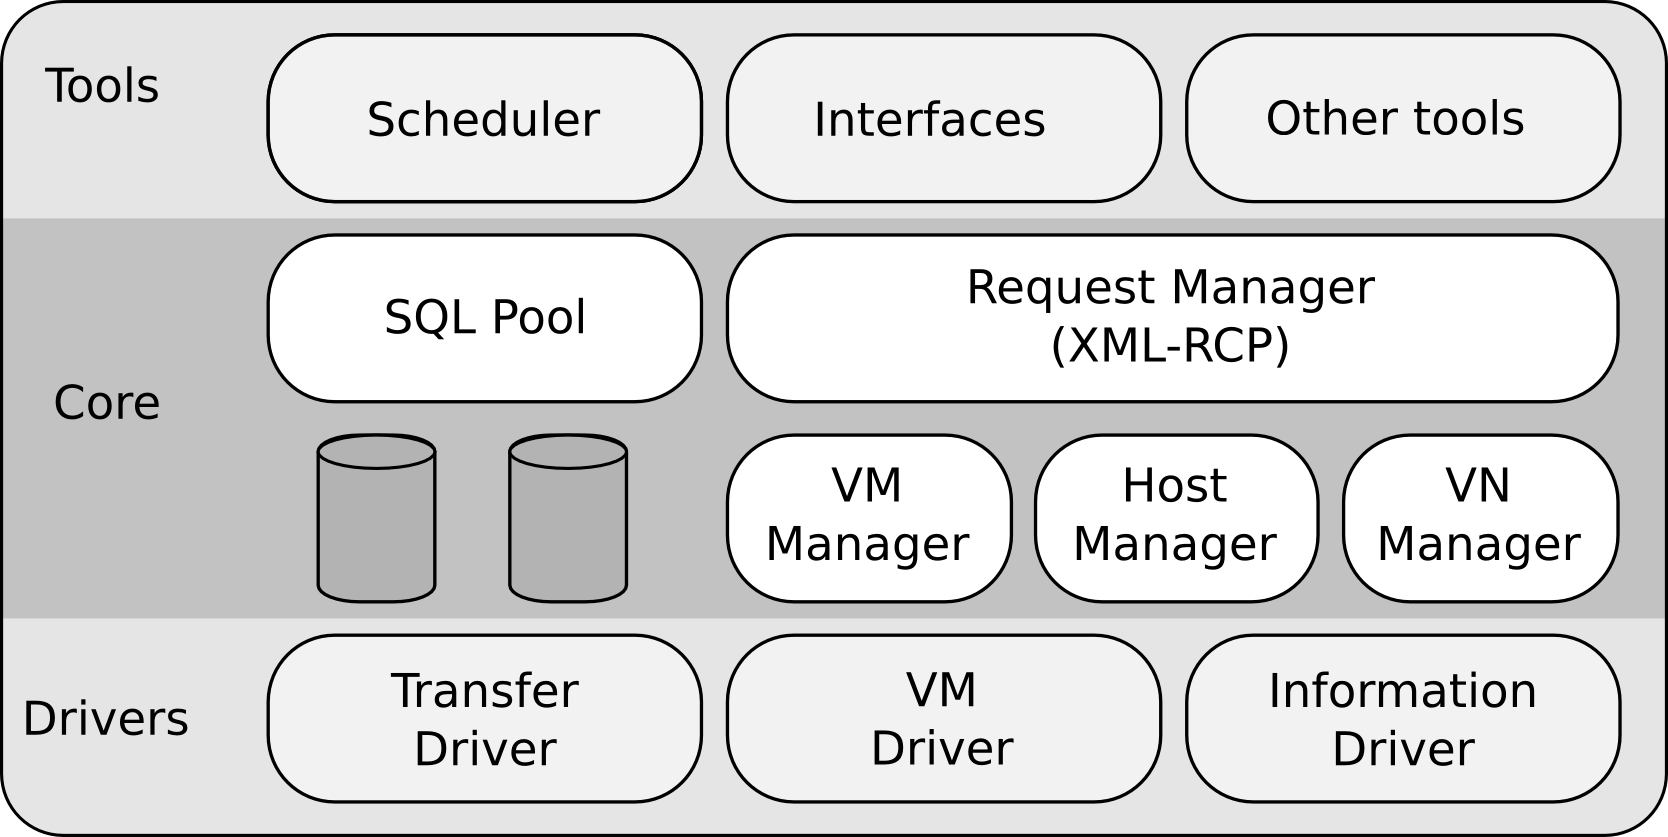
\includegraphics[scale=1]{one-architecture_2.png}
  \caption{OpenNebula architecture}
  \label{fig:open_arch}
\end{figure}

One important feature of the core module is the support of service deployment. The Request manager exposes a XML-RPC interface that decouples most of the functionality present in the core. It enables the creation of custom managers. As OpenNebula is in continuing development, it is expected that this API will support even more functionality. Currently, it is known that dynamic resource allocation is not supported yet. We'll discuss this issue on the next section, as this functionality is important for the advisor.

All these described activities are performed through pluggable drivers, present in the bottom layer. This modularity makes the system easier to extend and avoids tying it to any specific technology. The drivers shown in ~\ref{fig:open_arch}  address some particular areas, such as virtualization ( by controlling the hypervisor ), storage operations, gather monitoring information and authenticate user requests.

In the top layer there are both user interfaces to access OpenNebula, but also APIs extended from the XML-RPC, which can work between the core and other tools. Even more relevant for this paper is the OpenNebula's scheduler, also in this layer. Its job is to make VMs placement decisions ( i.e. it assigns physical machines for VMs ). It has access to all requests OpenNebula receives. Based on these requests, it keeps track on allocations and sends the appropriate deployment commands to OpenNebula's core. As other modules, it can be replaced by third party solutions, such as Haizea\footnote{http://haizea.cs.uchicago.edu/},  which offers more sophisticated placement policies. However, in this paper we will stick to the OpenNebula's default scheduler.

The scheduler already present in OpenNebula works only with immediate provisioning. Its concept is pretty straightforward, the resources are only provisioned at the moment they are required, if that's not possible, then the requirement is ignored. The requirements are done in a manual and static way, in which amount of resources, among other configurations, are defined in a file. The assignment is performed through a classification policy.  The administrator needs to set a \textit{RANK} variable, which defines which host is more suitable to host a VM. Each VM has its own \text{RANK}, and the scheduler assigns a host with the highest value for this variable to a VM. It's possible to define a VM template in OpenNebula, so you can share the same scheduling policy  to a group of VMs. For instance, here are some possible \textit{RANK} definitions, each one serving a specific policy:

\begin{itemize}
 \item Load-aware Policy
 \begin{itemize}
   \item \textbf{Heuristic:} Use nodes with less load;
   \item \textbf{Implementation:} Use nodes with more \textit{FREECPU} first.
    \item \textit{RANK} = \textit{FREECPU}

 \end{itemize}

  \item Striping policy
  \begin{itemize}
   \item \textbf{Heuristic:} Spread the VMs in the cluster node;
   \item \textbf{Implementation:} Use the nodes with less VMs running first.
   \item \textit{RANK} = "\textit{- RUNNING\_VMS}"
  \end{itemize}

\end{itemize}

